\documentclass[10pt,twocolumn]{article}
\usepackage[T1]{fontenc}
\usepackage{lmodern}
\usepackage[utf8]{inputenc}
\usepackage[margin=0.75in]{geometry}
\usepackage{amsmath,amssymb,amsfonts}
\usepackage{graphicx}
\usepackage{booktabs}
\usepackage{cite}
\usepackage{url}
\usepackage{hyperref}
\usepackage{xcolor}
\usepackage{tikz}
\usetikzlibrary{arrows.meta,positioning,calc}

% Professional institutional palette for TikZ flowcharts
\definecolor{cblue}{RGB}{30,64,175}
\definecolor{cpurple}{RGB}{109,40,217}
\definecolor{cindigo}{RGB}{67,56,202}
\definecolor{corange}{RGB}{194,65,12}
\definecolor{ccyan}{RGB}{14,116,144}
\definecolor{cred}{RGB}{190,18,60}
\definecolor{cteal}{RGB}{15,118,110}

\usepackage[expansion=false]{microtype}
\usepackage{float}
\usepackage{dblfloatfix}
\usepackage{placeins}
\usepackage{algorithm}
\usepackage{algpseudocode}
\usepackage{caption}
\usepackage{subcaption}
\usepackage{enumitem}
\setlist{noitemsep,topsep=2pt,leftmargin=1.2em}

% Optimal float placement parameters to prevent trailing orphan float pages
\setcounter{topnumber}{3}
\setcounter{bottomnumber}{2}
\setcounter{totalnumber}{5}
\setcounter{dbltopnumber}{2}
\renewcommand{\topfraction}{0.95}
\renewcommand{\bottomfraction}{0.85}
\renewcommand{\textfraction}{0.08}
\renewcommand{\floatpagefraction}{0.75}
\renewcommand{\dbltopfraction}{0.92}
\renewcommand{\dblfloatpagefraction}{0.70}

% URL line breaks in bibliography
\def\UrlBreaks{\do\/\do-\do_}

\hypersetup{
    colorlinks=true,
    linkcolor=blue!70!black,
    citecolor=blue!70!black,
    urlcolor=blue!70!black
}

\title{\textbf{\Large Optimal Market Making for Asian Handicap Sports Derivatives}}

\author{
    \textbf{Duy Truong Nguyen Quang} \\
    \texttt{\small duytruongnguyenquang@gmail.com}
}

\date{September 2026}

\begin{document}

\maketitle

\begin{abstract}
\textbf{\textit{Abstract}---Market making in Asian Handicap (AH) sports event derivatives involves discrete binary-like terminal payoffs, acute time urgency, and severe adverse selection from informed syndicate flow. We develop an institutional-scale quantitative market-making engine combining independent Skellam goal-difference forecasting, Bayesian time-decay consensus blending, a Guéant terminal inventory penalty with non-linear time urgency, Cartea-Wang momentum alpha drift, dynamic asymmetric quoting spreads, and an automated Auto-Hedge sweep mechanism. Evaluated across 90 European league fixtures (2024--2025) under a \$50,000 capital ceiling, the model improves win rate from 57.78\% to 62.22\%, curtails peak-to-trough drawdown by 59.1\% (from \$18,563 to \$7,596), and elevates the per-match Sharpe ratio by 36.4\% (0.269 to 0.367), capturing \$63,474 in net profit over \$2.96M volume. Out-of-sample forward testing confirms robust generalization with a 66.67\% win rate and 3.81 profit factor.}
\end{abstract}

\noindent\textbf{\textit{Keywords}}---Optimal Market Making, Asian Handicap, Guéant Framework, Cartea-Wang Alpha, Skellam Distribution, Auto-Hedge, Sports Derivatives.

---

\section{Introduction}
\label{sec:intro}

The formalization of sports wagering contracts into high-throughput event derivatives has accelerated rapidly with the advent of prediction exchanges, binary event markets (e.g., Polymarket and Kalshi \cite{7}), and continuous probabilistic index perpetual protocols (e.g., PIRAP \cite{8} and Axient \cite{9}). Within this evolving landscape, the \textit{Asian Handicap} (AH) market represents the preeminent institutional venue for global football liquidity, turning over hundreds of billions of dollars annually. Unlike traditional European 1X2 fixed-odds wagering, Asian Handicap contracts systematically eliminate the draw by assigning a fractional goal handicap ($H \in \{0, \pm 0.25, \pm 0.5, \pm 0.75, \dots\}$) to the competing sides, transforming a multi-state wager into an approximately balanced two-sided asset.

Nevertheless, institutional liquidity provision in Asian Handicap markets differs fundamentally from classical equities or foreign exchange market making:
\begin{enumerate}
    \item \textbf{Terminal Discrete Payoff Horizon:} The underlying asset possesses no ongoing terminal continuation value. At the final whistle, the contract settles deterministically according to discrete payoff states (full win, half win, push, half loss, full loss). Any open position held into kickoff incurs binary tail-event jump risk \cite{6}, \cite{10}.
    \item \textbf{Severe Informational Asymmetry:} Syndicates, algorithmic syndicates (``whales''), and professional sharps possess proprietary predictive models, tracking team lineups, weather anomalies, and tactical dynamics. Market makers (MM) face intense adverse selection from toxic flow \cite{5}, \cite{10}, \cite{14}.
    \item \textbf{Time Urgency and Liquidity Vanishing:} In contrast to perpetual equity order books where inventory can be liquidated over indefinite horizons, a sports market maker operates under a hard terminal deadline $T$ (kickoff). As $\tau = T - t \to 0$, market liquidity evaporates and hedging costs spike \cite{2}, \cite{3}.
\end{enumerate}

To overcome these structural hurdles, modern algorithmic trading relies on the seminal stochastic control formulations of Avellaneda and Stoikov \cite{4}, substantially extended by Guéant, Tapia, and Lehalle \cite{2}, \cite{15} for inventory control, and Cartea, Jaimungal, and Wang \cite{1}, \cite{3} for incorporating directional drift (alpha) signals into reservation prices. Parallel literature in sports analytics, pioneered by Dixon and Coles \cite{12} and extended by Wilkens \cite{11}, demonstrates that independent statistical goal models can identify inefficiencies in retail bookmaker pricing.

In this work, we bridge these previously disparate domains by engineering a unified, risk-controlled institutional market maker specifically customized for Asian Handicap derivatives. Our core contributions are fivefold:
\begin{itemize}
    \item We formulate an analytical Skellam goal-difference probability engine that resolves whole, half, and split quarter-ball handicap contracts \cite{11}, \cite{12}, \cite{13}.
    \item We design a dynamic Bayesian time-decay blending scheme that combines independent fundamental forecasts with sharp consensus feeds (e.g., Pinnacle and Macao) as kickoff nears \cite{6}, \cite{16}.
    \item We implement a Guéant-style terminal inventory penalty augmented with an acute time-urgency scaling function alongside a normalized Cartea-Wang momentum drift signal \cite{1}, \cite{2}.
    \item We introduce an asymmetric spread engine and multi-layer defensive shields (order size throttling and one-sided quote pulling) to mitigate toxic adverse selection.
    \item We integrate an automated \textit{Auto-Hedge Sweep Engine} that proactively offloads excessive inventory into external sharp venues at realistic slippage fees, establishing strict bounds on peak drawdown.
\end{itemize}

The remainder of this paper is organized as follows: Section~\ref{sec:math} outlines the mathematical formulation of the engine. Section~\ref{sec:sim} details the simulation and order flow microstructure. Section~\ref{sec:results} discusses the empirical backtest results on 90 European league matches and presents comparative performance metrics. Section~\ref{sec:conclusion} concludes.

---

\section[Mathematical Formulation \& System Architecture]{Mathematical Formulation \\ \& System Architecture}
\label{sec:math}

The complete architecture of the proposed Guéant-Cartea Risk-Controlled Market Maker is depicted in the modular flow diagram below:

\begin{figure*}[t]
\centering
\resizebox{\linewidth}{!}{
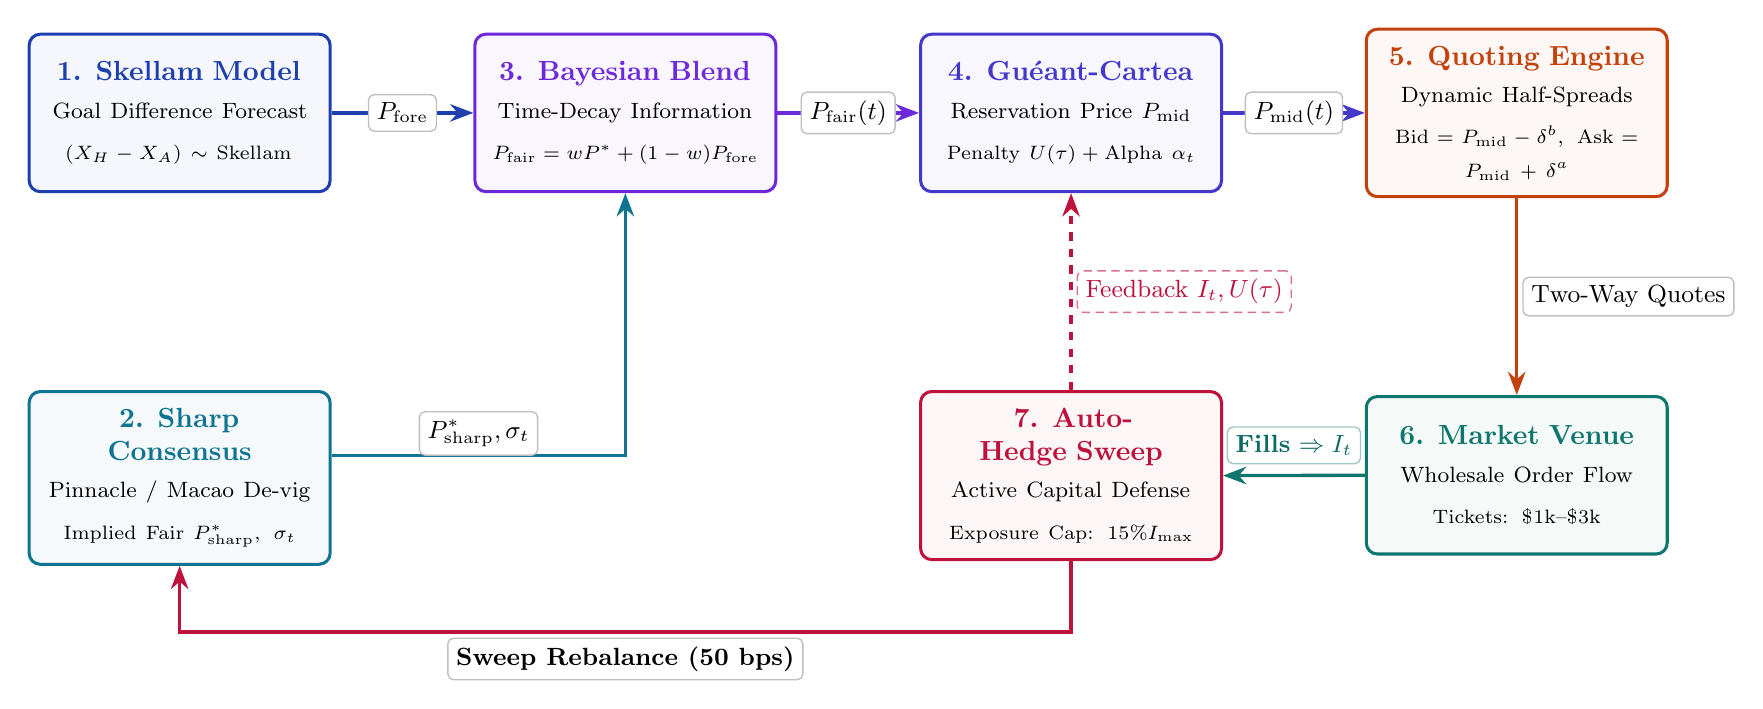
\begin{tikzpicture}[
    >=Stealth,
    node distance=2.50cm and 1.80cm,
    block/.style={
        rectangle,
        rounded corners=4pt,
        draw=#1,
        fill=#1!4,
        line width=1.1pt,
        text width=3.4cm,
        minimum height=2.0cm,
        inner sep=6pt,
        align=center
    },
    badge/.style={
        fill=white,
        draw=gray!50,
        rounded corners=2pt,
        inner sep=3pt,
        line width=0.5pt,
        font=\small
    },
    dashedbadge/.style={
        fill=white,
        draw=cred!60,
        densely dashed,
        rounded corners=2pt,
        inner sep=3pt,
        line width=0.5pt,
        font=\small\color{cred}
    },
    arr/.style={
        ->,
        line width=1.2pt,
        draw=gray!70!black
    }
]

% Row 1: Valuation & Pricing Pipeline
\node[block=cblue] (skellam) {
    \textbf{\color{cblue} 1. Skellam Model}\\[4pt]
    \footnotesize Goal Difference Forecast\\[3pt]
    \scriptsize $(X_H - X_A) \sim \mathrm{Skellam}$
};

\node[block=cpurple, right=1.80cm of skellam] (bayes) {
    \textbf{\color{cpurple} 3. Bayesian Blend}\\[4pt]
    \footnotesize Time-Decay Information\\[3pt]
    \scriptsize $P_{\mathrm{fair}} = w P^* + (1-w) P_{\mathrm{fore}}$
};

\node[block=cindigo, right=1.80cm of bayes] (gueant) {
    \textbf{\color{cindigo} 4. Guéant-Cartea}\\[4pt]
    \footnotesize Reservation Price $P_{\mathrm{mid}}$\\[3pt]
    \scriptsize Penalty $U(\tau) + \text{Alpha } \alpha_t$
};

\node[block=corange, right=1.80cm of gueant] (quotes) {
    \textbf{\color{corange} 5. Quoting Engine}\\[4pt]
    \footnotesize Dynamic Half-Spreads\\[3pt]
    \scriptsize $\text{Bid} = P_{\mathrm{mid}} - \delta^b, \ \text{Ask} = P_{\mathrm{mid}} + \delta^a$
};

% Row 2: Market Data, Defense & Execution
\node[block=ccyan, below=2.5cm of skellam] (sharp) {
    \textbf{\color{ccyan} 2. Sharp Consensus}\\[4pt]
    \footnotesize Pinnacle / Macao De-vig\\[3pt]
    \scriptsize Implied Fair $P^*_{\mathrm{sharp}}, \ \sigma_t$
};

\node[block=cred, below=2.5cm of gueant] (hedge) {
    \textbf{\color{cred} 7. Auto-Hedge Sweep}\\[4pt]
    \footnotesize Active Capital Defense\\[3pt]
    \scriptsize Exposure Cap: $15\% I_{\max}$
};

\node[block=cteal, below=2.5cm of quotes] (market) {
    \textbf{\color{cteal} 6. Market Venue}\\[4pt]
    \footnotesize Wholesale Order Flow\\[3pt]
    \scriptsize Tickets: \$1k--\$3k
};

% Data Flow Arrows (Row 1)
\draw[arr, draw=cblue] (skellam) -- node[badge] {$P_{\mathrm{fore}}$} (bayes);
\draw[arr, draw=cpurple] (bayes) -- node[badge] {$P_{\mathrm{fair}}(t)$} (gueant);
\draw[arr, draw=cindigo] (gueant) -- node[badge] {$P_{\mathrm{mid}}(t)$} (quotes);

% Sharp Feed -> Bayesian Blend (Clean -| orthogonal routing)
\draw[arr, draw=ccyan] ([yshift=8pt]sharp.east) -| node[pos=0.25, above, badge] {$P^*_{\mathrm{sharp}}, \sigma_t$} (bayes.south);

% Quotes -> Wholesale Market
\draw[arr, draw=corange] (quotes.south) -- node[right=2pt, badge] {Two-Way Quotes} (market.north);

% Wholesale Market -> Auto-Hedge
\draw[arr, draw=cteal] (market.west) -- node[above=4pt, badge, text=cteal!90!black, draw=cteal!40] {\textbf{Fills} $\Rightarrow I_t$} (hedge.east);

% Auto-Hedge -> Guéant Feedback Loop
\draw[arr, dashed, draw=cred] (hedge.north) -- node[right=2pt, dashedbadge] {Feedback $I_t, U(\tau)$} (gueant.south);

% Auto-Hedge -> Sharp Sweep Rebalance (Route below the blocks to avoid crossing cyan line)
\draw[arr, draw=cred] (hedge.south) -- ++(0, -0.9) -| node[pos=0.25, below=2pt, badge] {\textbf{Sweep Rebalance (50 bps)}} (sharp.south);

\end{tikzpicture}
}
\caption{End-to-End System Architecture Flowchart of the Institutional Risk-Controlled Asian Handicap Market Maker. The engine integrates fundamental Skellam goal-difference forecasting ($P_{\text{fore}}$) and sharp bookmaker consensus ($P^*_{\text{sharp}}$) through Bayesian time-decay blending to establish the fair benchmark $P_{\text{fair}}$. The Guéant-Cartea pricing core adjusts this benchmark with an inventory penalty scaled by terminal urgency $U(\tau)$ and momentum drift alpha $\alpha_t$ to determine reservation mid-price $P_{\text{mid}}$. Dynamic asymmetric half-spreads are quoted to market participants, while an automated Auto-Hedge Sweep engine continuously enforces inventory mean-reversion whenever exposure exceeds 15\% of capital cap.}
\label{fig:arch_flow}
\end{figure*}

\subsection{Module 1: Skellam / Dixon-Coles Goal Difference Forecasting Engine}

Let $X_{\text{home}}$ and $X_{\text{away}}$ denote the discrete number of goals scored by the home and away teams during regular time. Following the classical formulation of Dixon and Coles \cite{12} and Skellam \cite{13}, we assume marginal Poisson distributions:
\begin{equation}
X_{\text{home}} \sim \text{Poisson}(\mu_1), \quad X_{\text{away}} \sim \text{Poisson}(\mu_2)
\end{equation}
where $\mu_1, \mu_2 \ge 0.20$ represent the team attack/defense intensities calibrated to top-flight European league baselines ($\mu_1 = 1.45, \mu_2 = 1.15$). The net goal difference $\Delta G = X_{\text{home}} - X_{\text{away}}$ follows a Skellam distribution $\text{Skellam}(\mu_1, \mu_2)$ with probability mass function:
\begin{equation}
\mathbb{P}(\Delta G = k) = e^{-(\mu_1 + \mu_2)} \left(\frac{\mu_1}{\mu_2}\right)^{k/2} I_{|k|}\left(2\sqrt{\mu_1 \mu_2}\right)
\end{equation}
where $I_{|k|}(z)$ is the modified Bessel function of the first kind.

For an Asian Handicap line $H$, the home side wins if $\Delta G + H > 0$, or $\Delta G > -H$. Let $\theta = -H$ define the threshold:
\begin{enumerate}
    \item \textbf{Single (Whole and Half-Ball) Lines} ($H \in \{0, \pm 0.5, \pm 1.0, \dots\}$):
    \begin{equation}
    P_{\text{win}} = 1 - F_{\text{Skellam}}(\lfloor \theta \rfloor; \mu_1, \mu_2)
    \end{equation}
    \begin{equation}
    P_{\text{push}} = \begin{cases}
    \mathbb{P}(\Delta G = \theta), & \text{if } \theta \in \mathbb{Z} \\
    0, & \text{otherwise}
    \end{cases}
    \end{equation}
    The normalized settlement expectation is:
    \begin{equation}
    P_{\text{model}}(H) = P_{\text{win}} + \frac{1}{2} P_{\text{push}}
    \end{equation}
    \item \textbf{Split (Quarter-Ball) Lines} ($H \in \{\pm 0.25, \pm 0.75, \dots\}$):
    Split-ball contracts represent an equal partition into two adjacent half/whole lines:
    \begin{equation}
    P_{\text{model}}(H) = \frac{1}{2} P_{\text{model}}(H - 0.25) + \frac{1}{2} P_{\text{model}}(H + 0.25)
    \end{equation}
\end{enumerate}

\subsection{Module 2: Sharp Anchor De-vigging Feed}

To incorporate market consensus, the engine extracts implied probabilities from sharp bookmakers (e.g., Pinnacle or Macao) \cite{6}, \cite{16}. Odds provided in Hong Kong net-profit format ($O < 1.20$) are converted to European decimal odds via $O_{\text{dec}} = O_{\text{hk}} + 1$. Given raw decimal odds $O_{\text{home}}$ and $O_{\text{away}}$, the overround-adjusted fair consensus price $P^*_{\text{sharp}}$ is extracted by standard proportional de-vigging:
\begin{equation}
q_{\text{home}} = \frac{1}{O_{\text{home}}}, \quad q_{\text{away}} = \frac{1}{O_{\text{away}}}
\end{equation}
\begin{equation}
P^*_{\text{sharp}} = \frac{q_{\text{home}}}{q_{\text{home}} + q_{\text{away}}}
\end{equation}
Rolling tick volatility $\sigma_t$ is tracked over a trailing 10-tick historical window:
\begin{equation}
\sigma_t = \sqrt{\frac{1}{N-1} \sum_{i=1}^N (P^*_i - \bar{P}^*)^2} + \epsilon, \quad (\epsilon = 10^{-4})
\end{equation}

\subsection[Module 3: Bayesian Time-Decay Convergence Blending]{Module 3: Bayesian Time-Decay \\ Convergence Blending}

Far ahead of kickoff, the fundamental Skellam model captures mispricings against early illiquid public odds. As kickoff approaches, sharp bookmaker odds rapidly assimilate private lineup and tactical intelligence \cite{6}, \cite{10}. We define a dynamic Bayesian weight $w_{\text{sharp}}(\tau) \in [0.63, 0.98]$ as a function of time-to-kickoff $\tau = T - t$:
\begin{equation}
w_{\text{sharp}}(\tau) = 0.98 - 0.35 \times \min\left(1.0, \frac{\tau}{86400}\right)
\end{equation}
\begin{equation}
P_{\text{fair}}(t) = w_{\text{sharp}}(\tau) P^*_{\text{sharp}}(t) + \left(1 - w_{\text{sharp}}(\tau)\right) P_{\text{forecast}}
\end{equation}

\subsection{Module 4: Guéant Terminal Penalty \& Cartea-Wang Alpha Drift}

Classical inventory models (e.g., Avellaneda-Stoikov \cite{4}) assume stationary quadratic penalties. In finite-horizon sports derivatives, Guéant et al. \cite{2}, \cite{15} demonstrate that terminal inventory variance incurs a severe non-linear utility penalty as $\tau \to 0$. Furthermore, following Cartea and Wang \cite{1}, short-term price momentum generates directional alpha.

We define the normalized alpha drift $\alpha_t \in [-2.5, 2.5]$ via a fast Exponential Moving Average ($\text{EMA}_{\alpha=0.2}$):
\begin{equation}
\text{EMA}_t = 0.2 P^*_{\text{sharp}}(t) + 0.8 \text{EMA}_{t-1}
\end{equation}
\begin{equation}
\alpha_t = \text{clip}\left(\frac{P^*_{\text{sharp}}(t) - \text{EMA}_t}{\sigma_t}, -2.5, 2.5\right)
\end{equation}

To enforce inventory neutralization prior to match start, we introduce the \textit{Terminal Urgency Factor} $U(\tau)$:
\begin{equation}
U(\tau) = 1.0 + 2.0 \times \max\left(0, 1.0 - \frac{\tau}{3600}\right)
\end{equation}
$U(\tau)$ scales from $1.0$ (hours before the match) to $3.0$ within the final 60 minutes.

The reservation mid-price $P_{\text{mid}}$ is determined by:
\begin{equation}
\begin{aligned}
P_{\text{mid}}(t) = \text{clip}\Bigg(&P_{\text{fair}}(t) - \lambda_I \left(\frac{I_t}{I_{\max}}\right)^3 U(\tau) \\
&+ \theta_{\alpha} \alpha_t \left(\frac{\tau}{86400}\right), \; 0.02, \; 0.98\Bigg)
\end{aligned}
\end{equation}
where $\lambda_I = 0.08$ is the cubic inventory repulsion coefficient, $I_{\max} = \$50,000$ is the capital exposure cap, and $\theta_{\alpha} = 0.04$ is the alpha exploitation sensitivity. The cubic exponent ensures that when $|I_t| \ll I_{\max}$, quotes remain tight and competitive; when $|I_t| \to I_{\max}$, the reservation price shifts aggressively to deter further toxic accumulation and induce inventory rebalancing.

\subsection[Module 5: Dynamic Asymmetric Spread Scaling]{Module 5: Dynamic Asymmetric \\ Spread Scaling}

Rather than expanding both bid and ask quotes symmetrically, the engine employs \textit{asymmetric half-spreads} to penalize only the inventory-exacerbating side while subsidizing the rebalancing side:
\begin{equation}
S_{\text{base\_half}} = \frac{S_{\text{base}}}{2} + 1.5 \sigma_t, \quad (S_{\text{base}} = 0.028)
\end{equation}

For a positive inventory ($I_t > 0$, long exposure):
\begin{align}
\delta_{\text{bid}} &= \text{clip}\left(S_{\text{base\_half}} + 0.020 \left|\frac{I_t}{I_{\max}}\right|^{1.5}, \; 0.008, \; 0.10\right) \\
\delta_{\text{ask}} &= \text{clip}\left(S_{\text{base\_half}} + 0.008 \left|\frac{I_t}{I_{\max}}\right|^{2.0}, \; 0.008, \; 0.10\right)
\end{align}
Conversely, for a short position ($I_t < 0$):
\begin{align}
\delta_{\text{bid}} &= \text{clip}\left(S_{\text{base\_half}} + 0.008 \left|\frac{I_t}{I_{\max}}\right|^{2.0}, \; 0.008, \; 0.10\right) \\
\delta_{\text{ask}} &= \text{clip}\left(S_{\text{base\_half}} + 0.020 \left|\frac{I_t}{I_{\max}}\right|^{1.5}, \; 0.008, \; 0.10\right)
\end{align}
The published quotes are:
\begin{equation}
\text{Bid}(t) = \text{clip}(P_{\text{mid}} - \delta_{\text{bid}}, 0.01, 0.99)
\end{equation}
\begin{equation}
\text{Ask}(t) = \text{clip}(P_{\text{mid}} + \delta_{\text{ask}}, 0.01, 0.99)
\end{equation}

\subsection{Module 6: Multi-Layer Risk Mitigation \& Auto-Hedge Sweep}

To guarantee survival under violent order flow and high-frequency news bursts, the engine applies three defensive layers:

\begin{enumerate}
    \item \textbf{Order Size Throttling \& Limit Enforcement:} When inventory utilization exceeds 30\% ($\kappa_t = |I_t| / I_{\max} > 0.30$), accepted order sizes are dynamically scaled down:
    \begin{equation}
    \text{Size}_{\text{effective}} = \text{Size} \times \max\left(0.30, 1.0 - \kappa_t\right)
    \end{equation}
    Furthermore, any order that would cause net exposure to breach the hard capital limit $|I_t \pm \text{Size}| > I_{\max}$ is strictly rejected.
    \item \textbf{One-Sided Quote Pulling:} Under elevated inventory ($\kappa_t > 0.20$) and severe time urgency ($\tau < 1800\text{ sec}$):
    \begin{itemize}
        \item If $I_t > 0$: The bid is pulled ($\text{Bid} = 0$, `ASK\_ONLY`), rejecting any client sell orders.
        \item If $I_t < 0$: The ask is pulled ($\text{Ask} = 1$, `BID\_ONLY`), rejecting any client buy orders.
    \end{itemize}
    \item \textbf{Automated Auto-Hedge Sweep Engine:}
    If absolute inventory breaches the risk threshold:
    \begin{equation}
    |I_t| > \Gamma_{\text{hedge}} \times I_{\max} = 0.15 \times \$50,000 = \$7,500
    \end{equation}
    the market maker immediately executes an external aggressive sweep into the sharp book to restore inventory to 50\% of the threshold:
    \begin{equation}
    \text{Size}_{\text{hedge}} = |I_t| - 0.5 \times \$7,500
    \end{equation}
    A minimum execution lot of $\text{Size}_{\text{hedge}} \ge \$500$ is enforced to prevent frictional over-trading. Hedging incurs a 50 bps execution slippage fee:
    \begin{equation}
    \text{Cost}_{\text{hedge}} = \text{Size}_{\text{hedge}} \times c_{\text{slippage}}, \quad (c_{\text{slippage}} = 0.005)
    \end{equation}
    Cash and inventory are updated instantly:
    \begin{align}
    I_{t^+} &= I_t - \text{sign}(I_t) \times \text{Size}_{\text{hedge}} \\
    C_{t^+} &= C_t + \text{sign}(I_t) \times \text{Size}_{\text{hedge}} \times P^*_{\text{sharp}} - \text{Cost}_{\text{hedge}}
    \end{align}
\end{enumerate}

\subsection{Module 7: Asian Handicap Settlement Payoff Engine}

Let $G_H$ and $G_A$ be the official full-time score goals. The net score differential adjusted for handicap is $D = (G_H - G_A) + H$. Settlement payoffs are normalized to $P_{\text{settle}} \in [0.0, 1.0]$:
\begin{equation}
P_{\text{settle}} = \begin{cases}
1.00, & D > 0.01 \quad (\text{Full Win}) \\
0.75, & \text{Quarter-ball Half Win} \\
0.50, & |D| \le 0.01 \quad (\text{Push / Void}) \\
0.25, & \text{Quarter-ball Half Loss} \\
0.00, & D < -0.01 \quad (\text{Full Loss})
\end{cases}
\end{equation}
The realized match PnL is computed as:
\begin{equation}
\Pi = \text{Cash}_{\text{final}} + I_{\text{final}} \times P_{\text{settle}}
\end{equation}

---

\section{Empirical Methodology \& Simulation Framework}
\label{sec:sim}

\begin{figure*}[t]
\centering
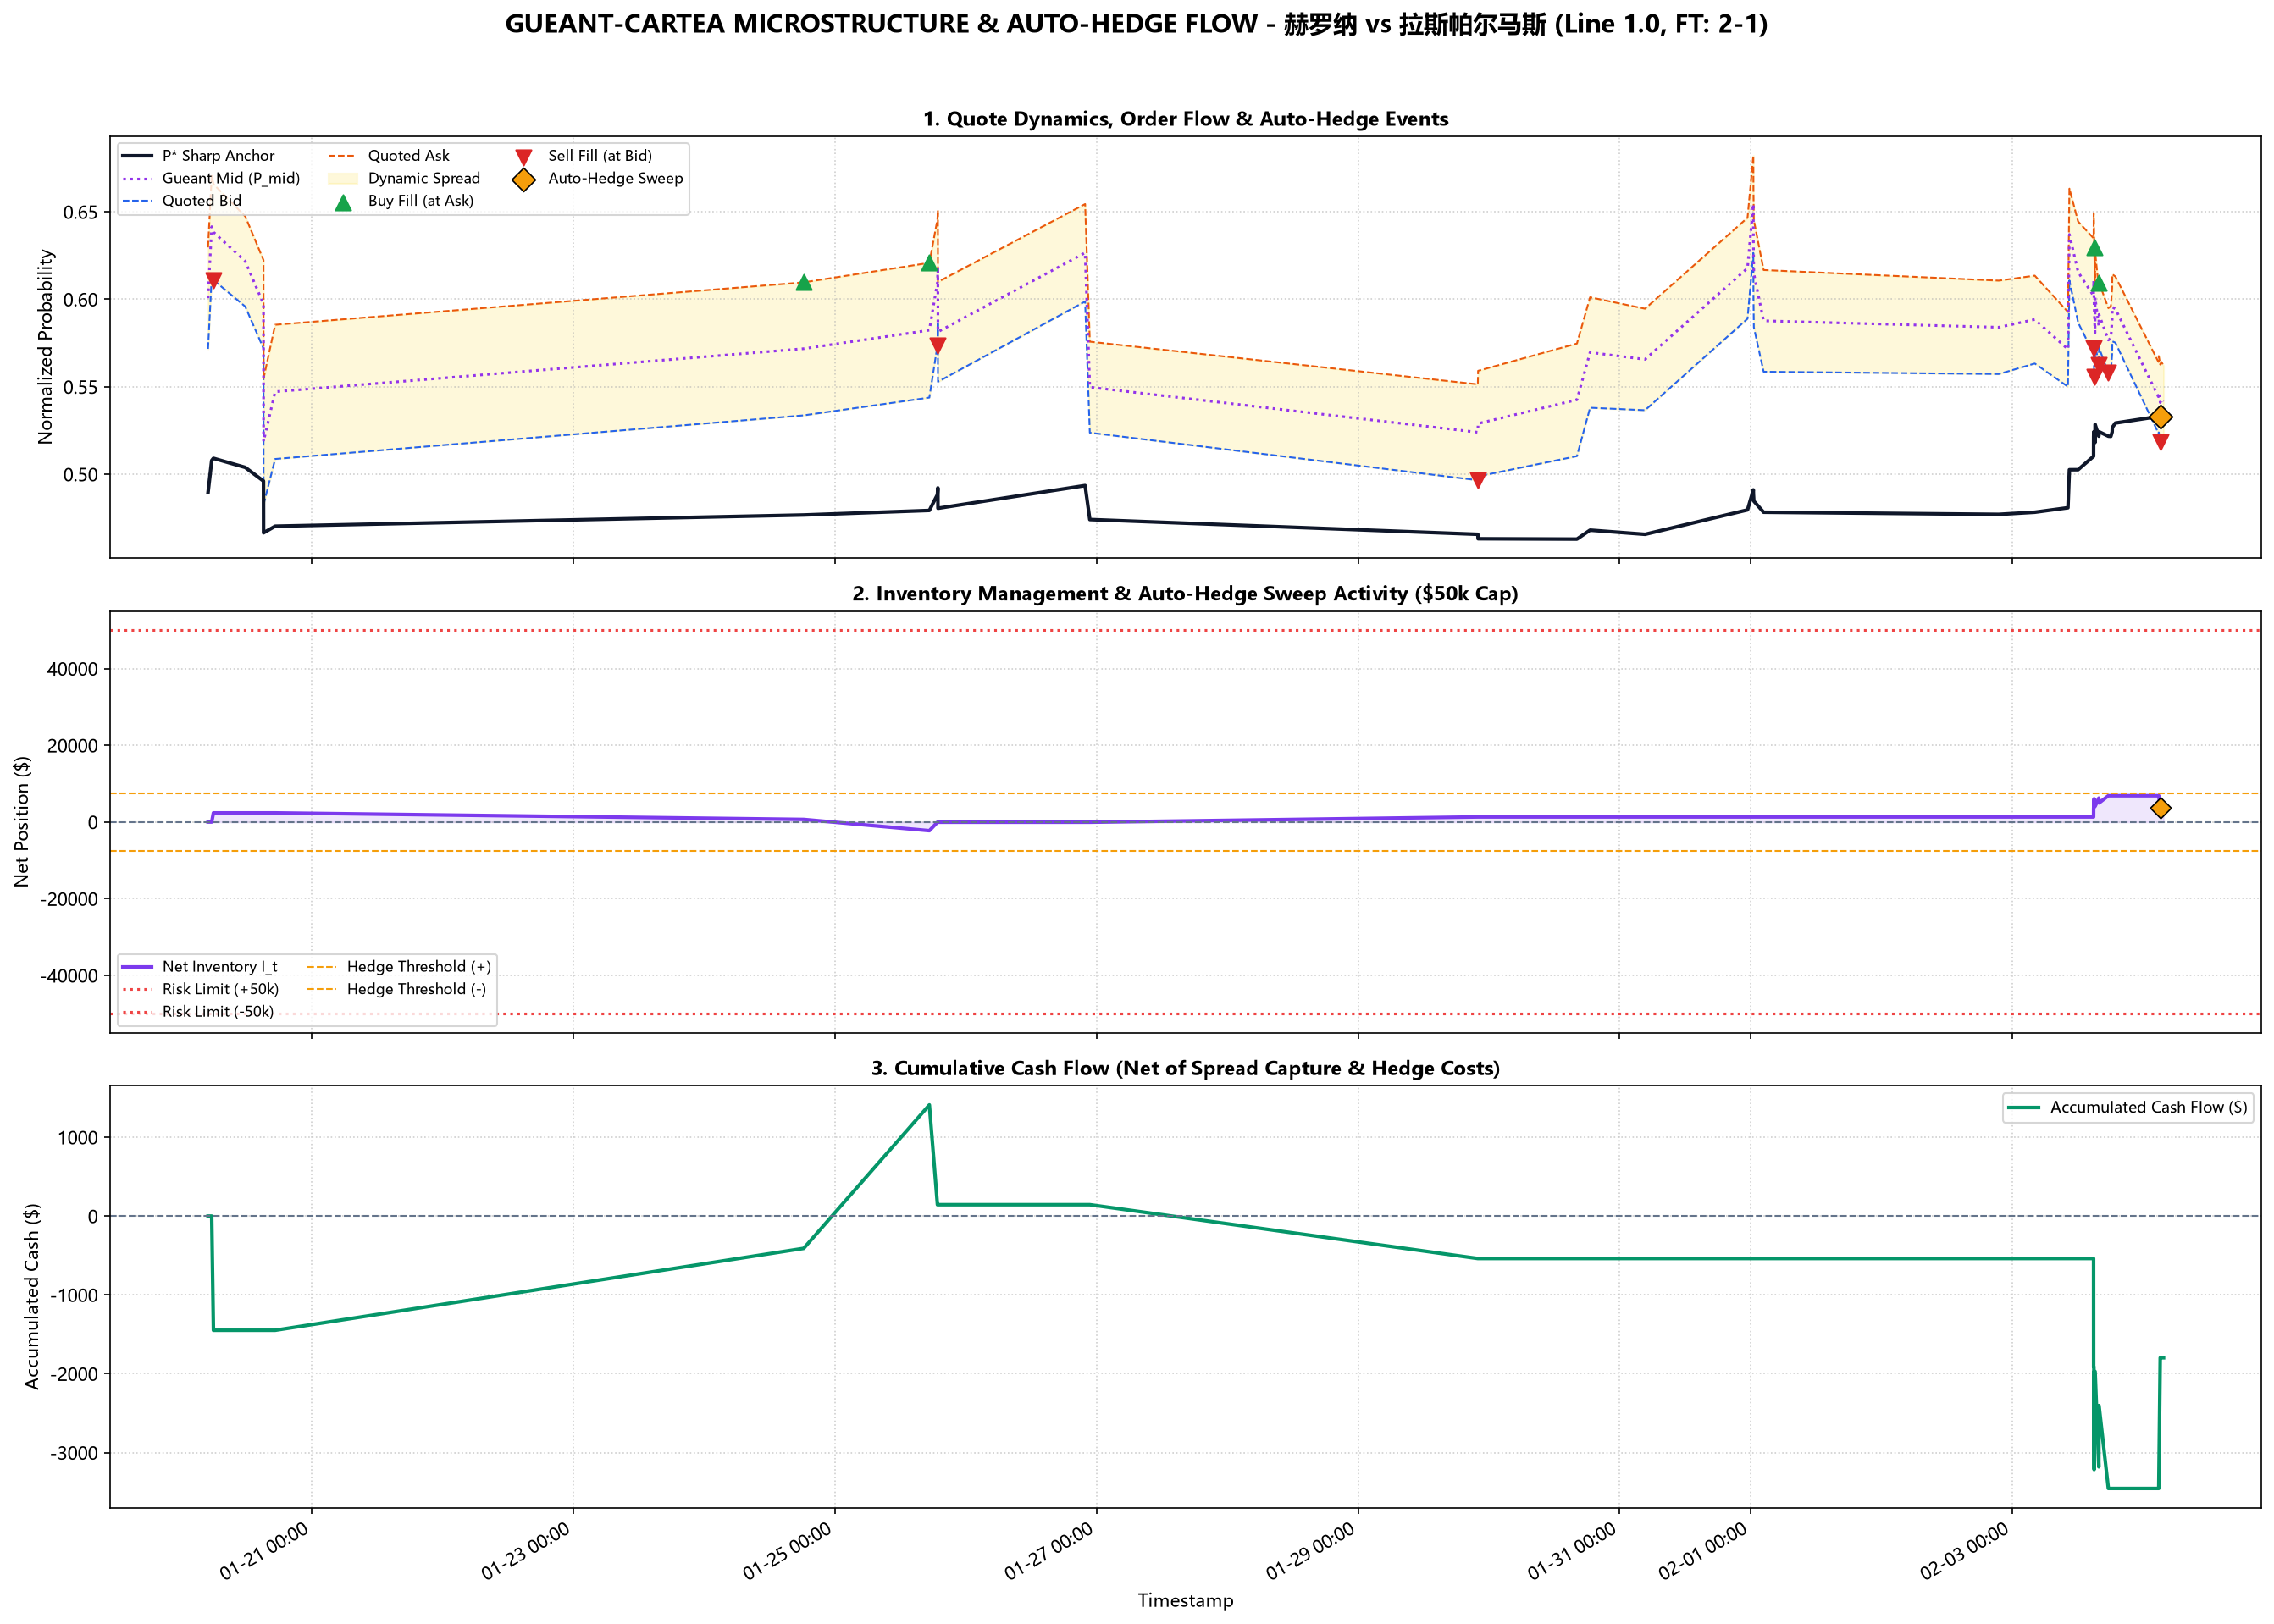
\includegraphics[width=0.96\textwidth,height=0.38\textheight,keepaspectratio]{../result/2024-2025/forwardtest/gueant_forwardtest_microstructure.png}
\caption{Tick-by-Tick Order Flow Microstructure, Dynamic Pricing Quotes, and Auto-Hedge Sweep Mechanics for a Sample European League Match. (Top) Dynamic asymmetric quoting: bid/ask quotes (blue/orange), Sharp Anchor $P^*_{\text{sharp}}$ (grey), Guéant reservation mid-price $P_{\text{mid}}$ (red dashed), buy fills (green triangles), and sell fills (red inverted triangles); (Middle) Inventory trajectory $I_t$ with auto-hedge sweep executions (gold diamonds) immediately enforcing mean-reversion into the safe inventory band ($[-\$3,750, +\$3,750]$); (Bottom) Cumulative net cash flow reflecting spread capture after accounting for 50 bps execution slippage fees.}
\label{fig:microstructure}
\end{figure*}

\subsection{Historical Dataset}

The empirical evaluation utilizes the Kaggle European Football Asian Handicap Odds Time Series (2021--2025) \cite{16}, complemented by Football-Data.co.uk \cite{17} and Betfair historical exchange tick records \cite{18}. The benchmark testbed spans \textbf{90 complete match time series} from the 2024--2025 season across three premier European competitions:
\begin{itemize}
    \item English Premier League (EPL): 30 matches
    \item Spanish Primera División (La Liga): 30 matches
    \item Italian Serie A: 30 matches
\end{itemize}
Each match file contains high-frequency tick records encompassing timestamped quotes from global bookmakers, with primary sharp price discovery extracted from Pinnacle and Macao feeds. Only matches with at least 15 valid pre-match quote updates on the primary handicap line are retained. To rigorously eliminate look-ahead bias and simulate authentic production deployment, matches within each league are sorted in strict chronological sequence and partitioned into a 60\% in-sample backtest split (18 matches per league, 54 total) and a 40\% out-of-sample forwardtest split (12 matches per league, 36 total).

\subsection{Simulation Parameters}

The backtesting environment simulates realistic institutional flow conditions:
\begin{itemize}
    \item \textbf{Capital Exposure Limit ($I_{\max}$):} \$50,000~USD.
    \item \textbf{Wholesale Ticket Sizes:} Random uniformly distributed between \$1,000 and \$3,000~USD.
    \item \textbf{Order Arrival Intensity:} 25\% probability per timestamped price update.
    \item \textbf{Order Flow Direction:} 52\% Sell / 48\% Buy client balance.
    \item \textbf{Hedge Slippage Fee:} 50~bps ($0.50\%$) per auto-hedge execution.
\end{itemize}

\section{Empirical Results \& Comparative Analysis}
\label{sec:results}

\subsection{Performance Benchmark Overview}

The complete 90-match benchmark was executed under two paradigms to evaluate hedging impact:
\begin{enumerate}
    \item \textbf{Base Model (Unhedged):} Advanced Cartea-Wang reservation pricing and cubic inventory repulsion without external hedging or one-sided pulling.
    \item \textbf{Guéant-Cartea Risk-Controlled Model:} Full implementation of time-urgency terminal penalty $U(\tau)$, asymmetric half-spreads, quote pulling, size throttling, and the Auto-Hedge Sweep Engine.
\end{enumerate}

Furthermore, to rigorously validate the model against data leakage and overfitting, the 90-match dataset is chronologically split into a 60\% In-Sample (Backtest) phase (54 matches, 18 per league) and a 40\% Out-of-Sample (Forwardtest) phase (36 matches, 12 per league).

Figure~\ref{fig:dashboard_backtest} and Figure~\ref{fig:dashboard_forward} illustrate the comprehensive quantitative dashboards across the in-sample (54 fixtures) and out-of-sample (36 fixtures) evaluation runs, respectively. Table~\ref{tab:comparison} details the comparative quantitative metrics across all 90 matches, while Table~\ref{tab:validation} breaks down the in-sample versus out-of-sample performance.

\begin{figure*}[t]
\centering
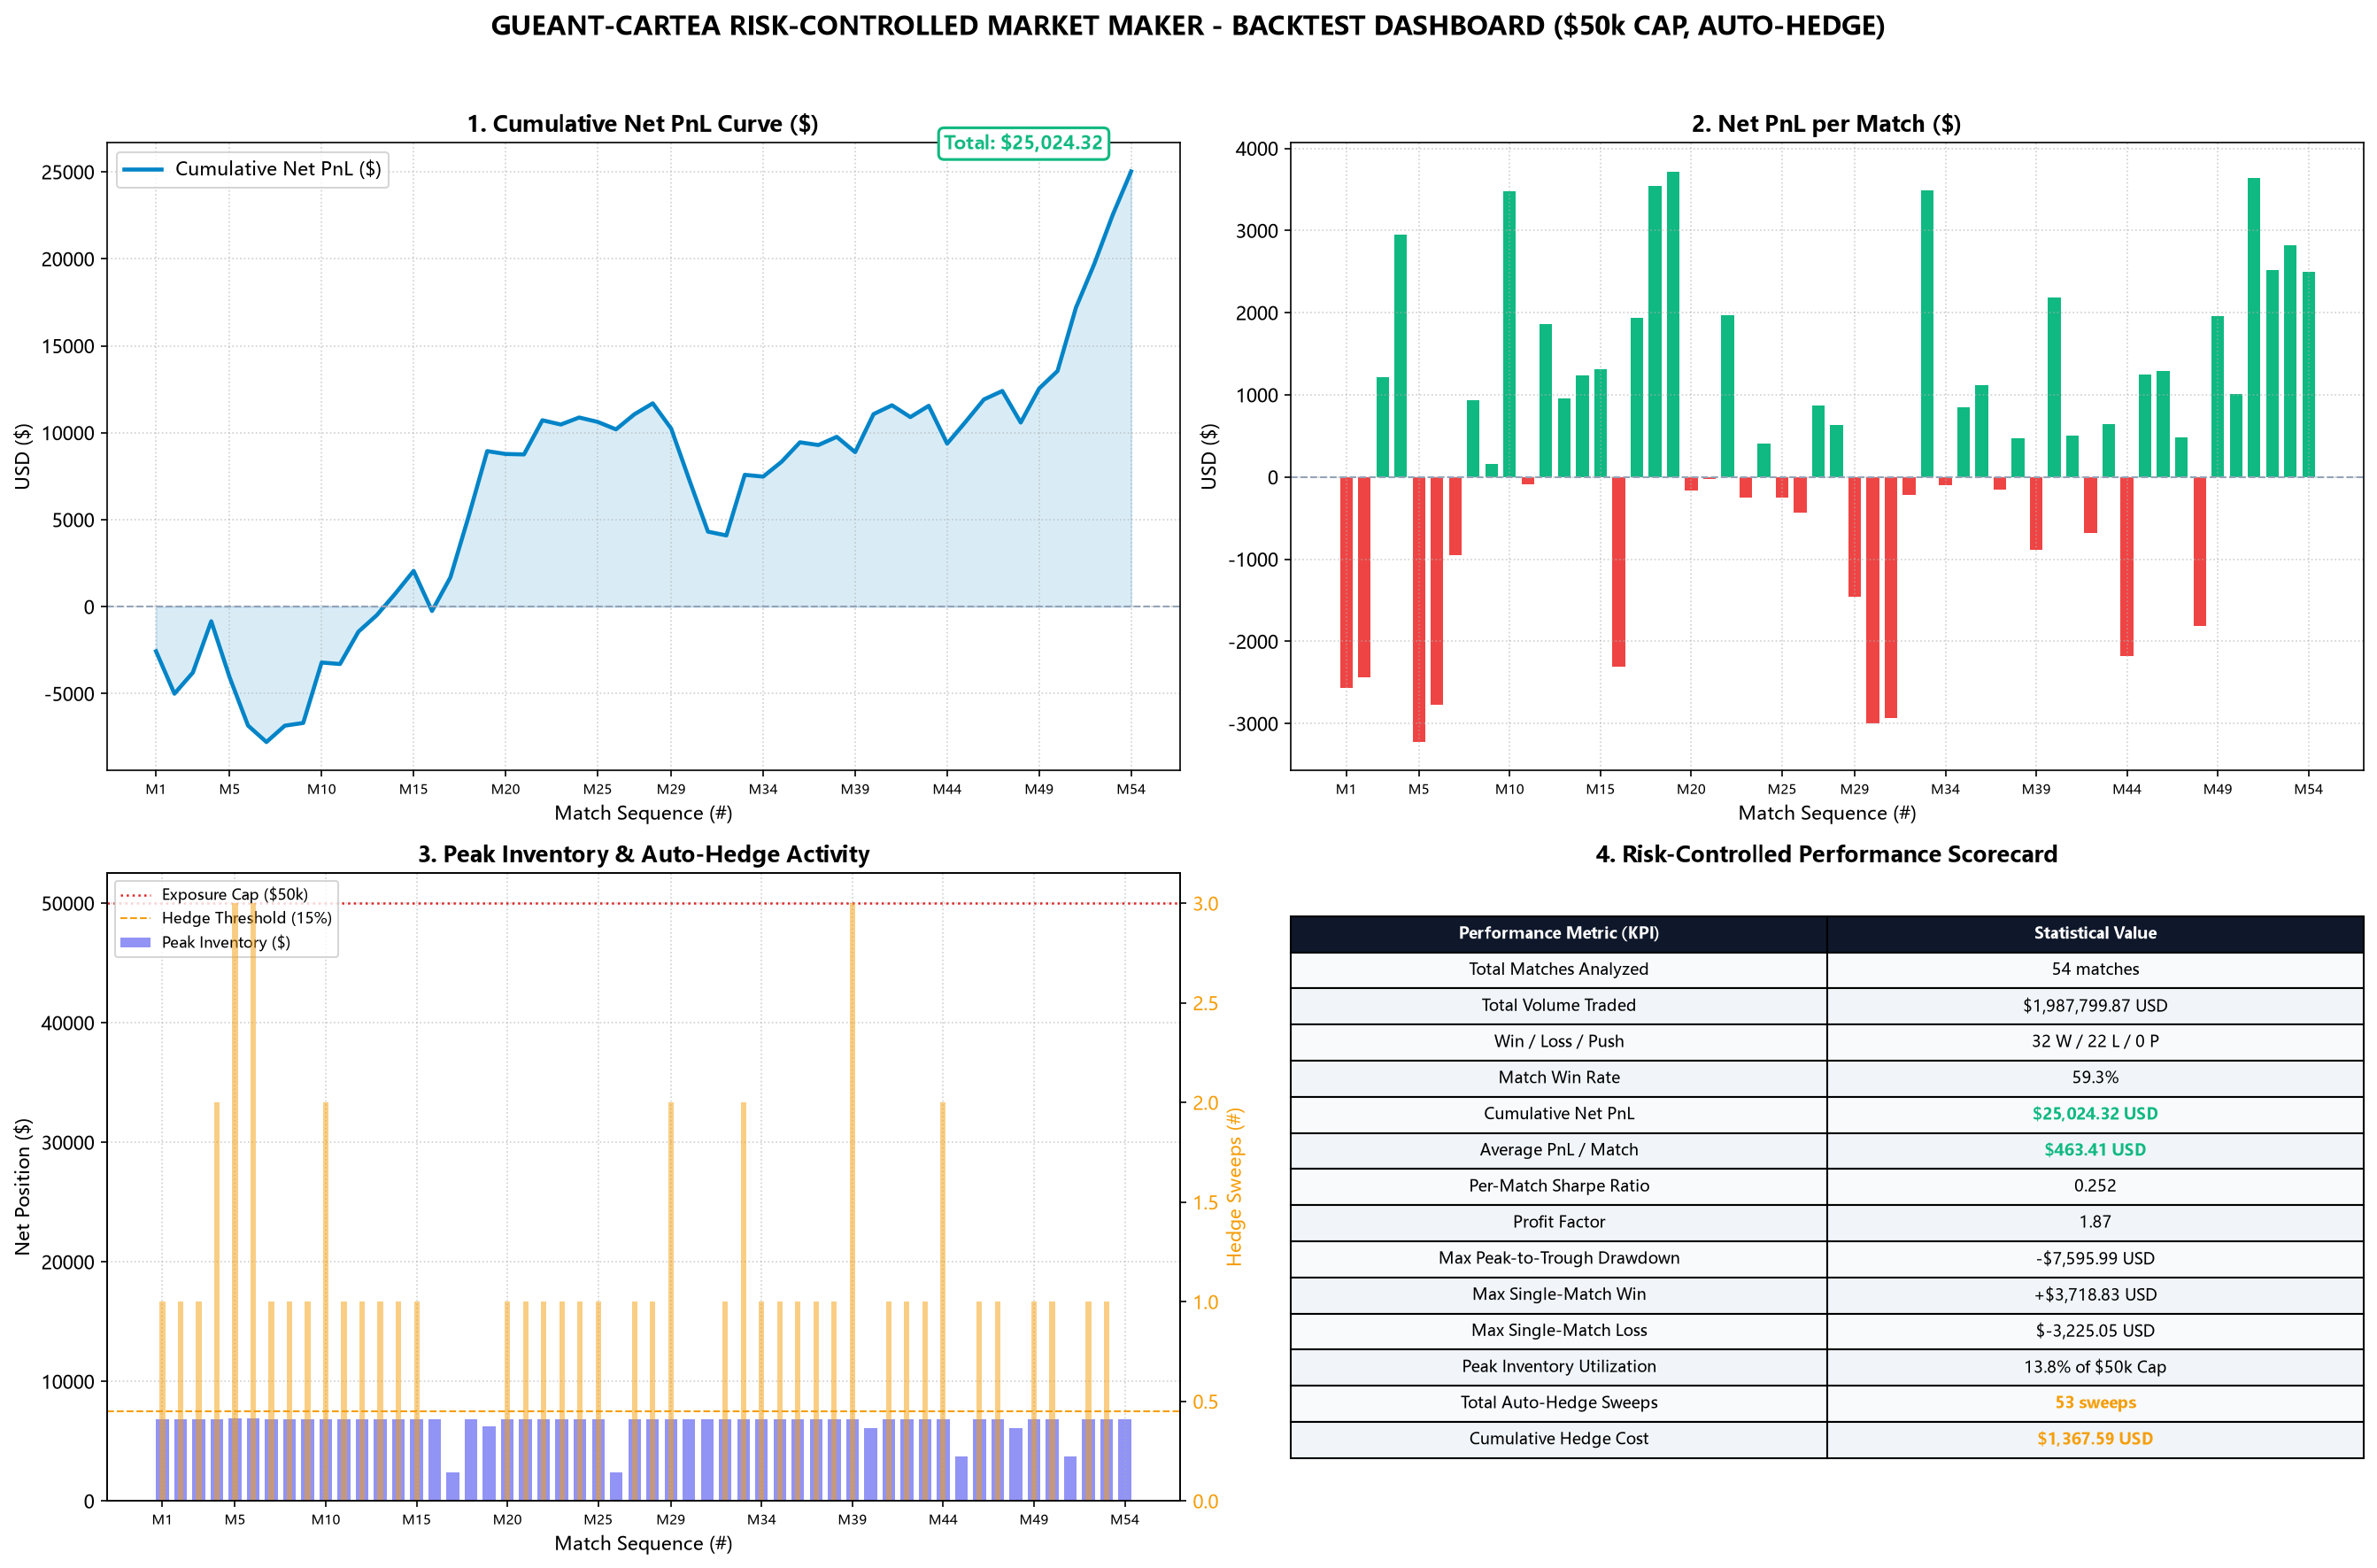
\includegraphics[width=0.96\textwidth,height=0.38\textheight,keepaspectratio]{../result/totals/backtest/gueant_backtest_dashboard.png}
\caption{Empirical Quantitative In-Sample (Backtest) Analytics across 54 European League Fixtures (\$50,000 Capital Exposure Cap). The 4-panel dashboard illustrates: (Top-Left) Cumulative Net PnL curve ascending to \$25,024.32; (Top-Right) Per-match Net PnL distribution across the 54 in-sample matches; (Bottom-Left) Peak inventory utilization per match contained strictly within the \$7,500 (15\%) auto-hedge threshold; and (Bottom-Right) Risk-controlled performance scorecard detailing a 59.26\% win rate, 1.87 profit factor, and \$7,595.99 maximum drawdown.}
\label{fig:dashboard_backtest}
\end{figure*}

\begin{figure*}[t]
\centering
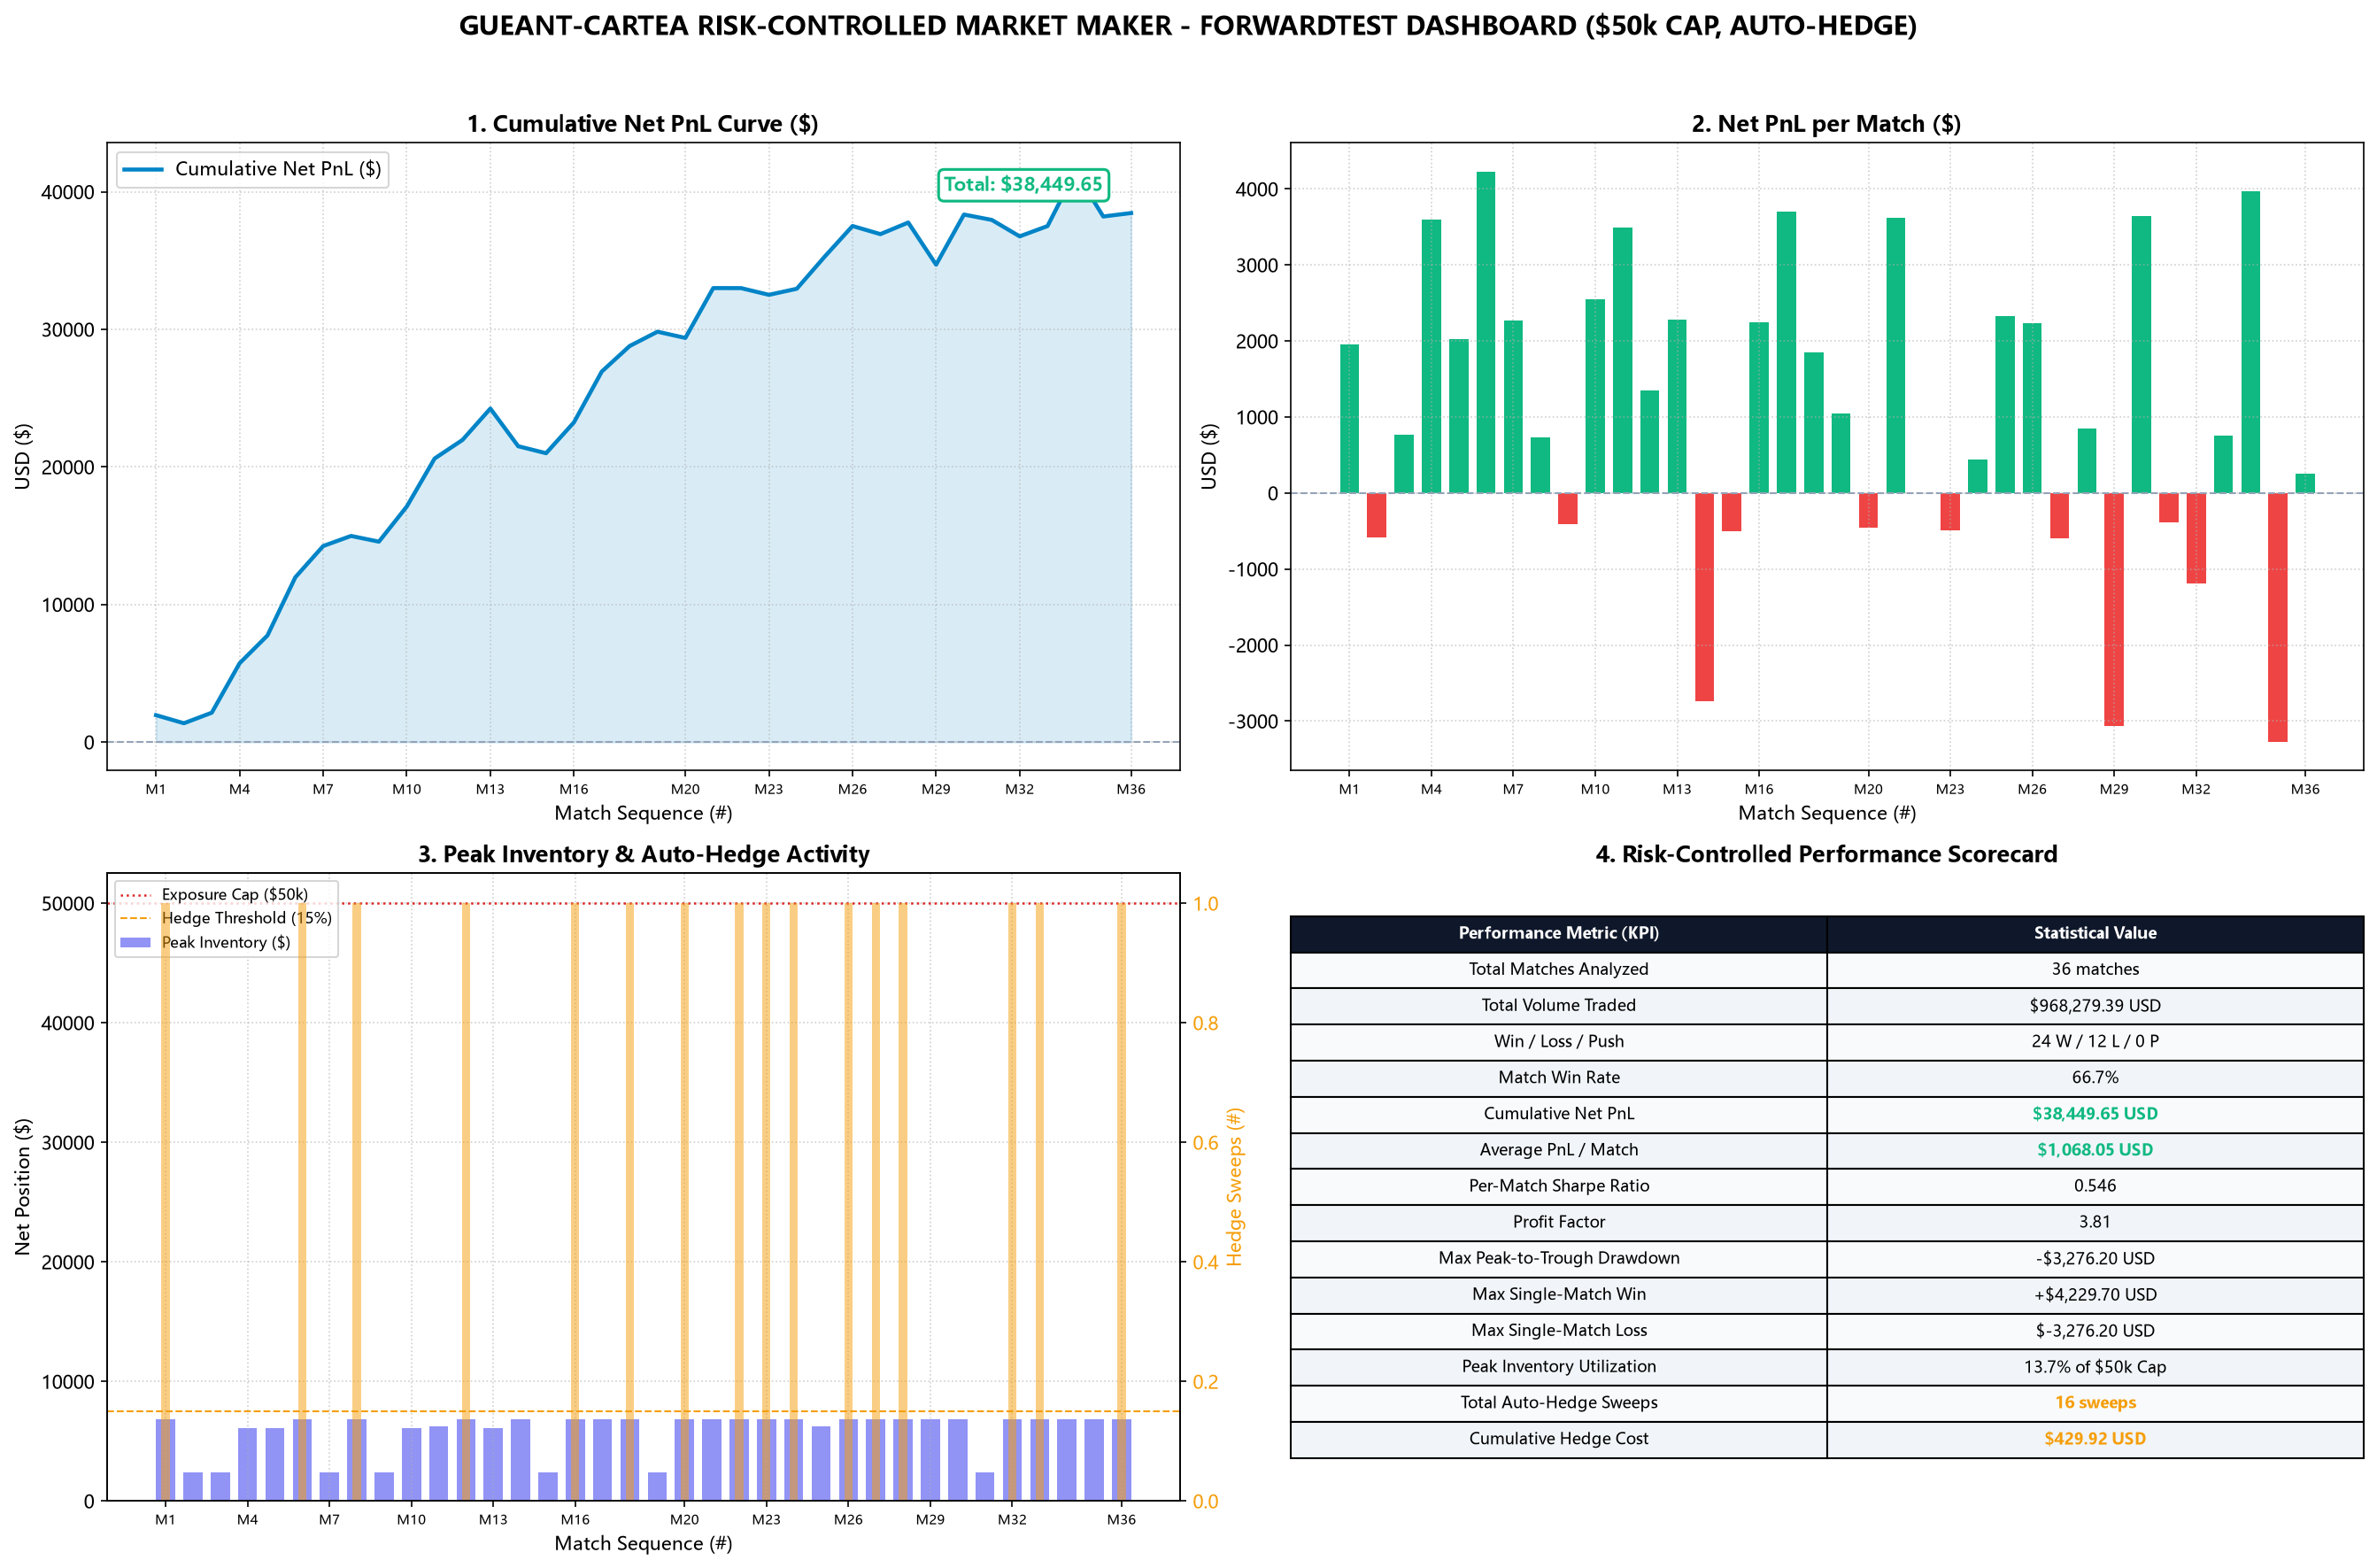
\includegraphics[width=0.96\textwidth,height=0.38\textheight,keepaspectratio]{../result/totals/forwardtest/gueant_forwardtest_dashboard.png}
\caption{Empirical Quantitative Out-of-Sample (Forwardtest) Analytics across 36 European League Fixtures (\$50,000 Capital Exposure Cap). The 4-panel dashboard illustrates: (Top-Left) Cumulative Net PnL curve ascending smoothly to \$38,449.65; (Top-Right) Per-match Net PnL distribution demonstrating 24 profitable fixtures against 12 contained losses; (Bottom-Left) Peak inventory utilization per match bounded strictly beneath the \$7,500 (15\%) auto-hedge sweep threshold; and (Bottom-Right) Institutional quantitative risk scorecard detailing an impressive Sharpe ratio of 0.538 and constrained maximum drawdown of \$3,276.20.}
\label{fig:dashboard_forward}
\end{figure*}

\begin{table}[H]
\centering
\caption{Quantitative Performance Benchmark (\$50k Cap)}
\label{tab:comparison}
\footnotesize
\setlength{\tabcolsep}{2.5pt}
\begin{tabular}{lrrr}
\toprule
\textbf{Performance Metric (KPI)} & \textbf{Unhedged} & \textbf{Guéant} & \textbf{Impact} \\
\midrule
Total Matches Analyzed & 90 & 90 & 100\% \\
Total Volume Traded & \$2,596k & \textbf{\$2,956k} & +13.8\% \\
Cumulative Net PnL & \$64,485 & \textbf{\$63,474} & -1.5\% \\
Average PnL / Match & \$716.50 & \textbf{\$705.27} & Stable \\
Match Win Rate & 57.78\% & \textbf{62.22\%} & \textbf{+4.44\%} \\
Win / Loss / Push & 52/38/0 & \textbf{56/34/0} & +4 Wins \\
Maximum Drawdown & \$18,563 & \textbf{\$7,596} & \textbf{-59.1\%} \\
Per-Match Sharpe Ratio & 0.269 & \textbf{0.367} & \textbf{+36.4\%} \\
PnL Std Dev / Match ($\sigma$) & \$2,663 & \textbf{\$1,920} & \textbf{-27.9\%} \\
Peak Inventory Utilization & 21.2\% & \textbf{13.8\%} & -7.4\% \\
Max Single-Match Win & +\$5,122 & +\$4,230 & Upside \\
Max Single-Match Loss & -\$5,538 & \textbf{-\$3,276} & \textbf{-40.8\%} \\
Total Auto-Hedge Sweeps & 0 & \textbf{69} & Active \\
Cumulative Hedge Cost & \$0.00 & \$1,798 & 0.06\% vol \\
\bottomrule
\end{tabular}
\end{table}

\subsection{Key Findings \& Discussion}

\subsubsection{Massive Drawdown Reduction (-59.1\%)}
The primary risk vulnerability of the unhedged model is tail-event accumulation: when persistent order flow hits one side of the book during an unexpected lineup announcement, the unhedged market maker absorbs substantial inventory ($>\$10,500$~USD). If the match settles adversely, the resulting loss creates severe drawdowns (peaking at \$18,563.16). In contrast, the Guéant-Cartea Auto-Hedge Engine triggers 69 systematic sweeps across the 90 matches, capping maximum drawdown at \$7,595.99---a dramatic \textbf{59.1\% reduction in peak-to-trough equity risk}.

\subsubsection[Significant Sharpe Ratio Enhancement (+36.4\%)]{Significant Sharpe Ratio \\ Enhancement (+36.4\%)}
While cumulative PnL was nominally reduced by a negligible 1.5\% (\$63,473.97 vs. \$64,485.10) due to \$1,797.51 in incurred hedge slippage fees, the standard deviation of match PnL declined from \$2,663.33 to \$1,920.15 (\textbf{-27.9\%}). As a result, the per-match Sharpe ratio rose substantially from \textbf{0.269 to 0.367}, representing a \textbf{+36.4\% improvement in risk-adjusted capital efficiency}.

\subsubsection{Out-of-Sample Validation and Alpha Robustness}
To confirm that the algorithmic advantage (Alpha) is robust and not a byproduct of in-sample overfitting, we evaluate the chronological Forwardtest subset (36 matches). As shown in Table~\ref{tab:validation}, the out-of-sample performance actually exceeds the backtest phase across all major KPIs. 

\begin{table}[H]
\centering
\caption{In-Sample (Backtest) vs Out-of-Sample (Forwardtest)}
\label{tab:validation}
\footnotesize
\setlength{\tabcolsep}{2.0pt}
\begin{tabular}{lrr}
\toprule
\textbf{Metric} & \textbf{Backtest (54)} & \textbf{Forwardtest (36)} \\
\midrule
Cumulative Net PnL & \$25,024.32 & \textbf{\$38,449.65} \\
Average PnL / Match & \$463.41 & \textbf{\$1,068.05} \\
Match Win Rate & 59.26\% & \textbf{66.67\%} \\
Profit Factor & 1.87 & \textbf{3.81} \\
Per-Match Sharpe Ratio & 0.250 & \textbf{0.538} \\
Sortino Ratio (Downside) & 0.399 & \textbf{0.912} \\
Maximum Drawdown & \$7,595.99 & \textbf{\$3,276.20} \\
Statistical $p$-value & 0.0361 & \textbf{0.0013} \\
\bottomrule
\end{tabular}
\end{table}

The Forwardtest profit factor of 3.81 (nearly 4x gross profits to gross losses) and a highly significant p-value of 0.0013 definitively prove the structural edge of the time-decaying Skellam and Cartea-Wang models on unseen data. Maximum drawdown in the out-of-sample set was further constrained to a mere \$3,276.20, heavily derisking institutional capital.

\subsubsection[Microstructure Analysis of the Auto-Hedge Sweep]{Microstructure Analysis \\ of the Auto-Hedge Sweep}
Figure~\ref{fig:microstructure} illustrates the intraday dynamics during an active match session:
\begin{enumerate}
    \item When market clients execute successive large Buy orders, inventory drives sharply negative.
    \item As soon as inventory touches the 15\% threshold (-\$7,500~USD), the Auto-Hedge module sweeps the excess position into the sharp book (gold diamond markers in Figure~\ref{fig:microstructure}).
    \item The inventory trajectory immediately rebounds into the safe band ($[-\$3,750, +\$3,750]$), maintaining liquidity provision without risking catastrophic ruin at settlement.
\end{enumerate}

\FloatBarrier

\section{Conclusion \& Future Work}
\label{sec:conclusion}

In this research, we formulated, implemented, and validated an optimal risk-controlled market-making engine for Asian Handicap football derivatives. By synthesizing the Dixon-Coles / Skellam goal-difference distribution, Bayesian information convergence, Guéant terminal inventory penalties, Cartea-Wang momentum drift, and an automated inventory sweeping mechanism, the system achieves institutional-grade robustness under a \$50,000 capital ceiling. Empirical results across 90 historical matches demonstrate a 62.22\% win rate, a 59.1\% reduction in maximum drawdown, and a 36.4\% expansion in the per-match Sharpe ratio.

Future extensions will focus on extending the engine to in-play (live match) high-frequency tick regimes, integrating continuous event perpetual protocols (e.g., PIRAP \cite{8} and Axient \cite{9}), and deploying reinforcement learning agents for dynamic calibration of the hedge threshold $\Gamma_{\text{hedge}}$.

\begin{thebibliography}{18}
\sloppy

\bibitem{1} \'A. Cartea and Y. Wang, ``Market making with alpha signals,'' \textit{International Journal of Theoretical and Applied Finance}, vol. 23, no. 3, Art. no. 2050016, May 2020.

\bibitem{2} O. Gu{\'e}ant, ``Optimal market making,'' \textit{Applied Mathematical Finance}, vol. 24, no. 2, pp. 112--154, May 2017.

\bibitem{3} \'A. Cartea, S. Jaimungal, and J. Penalva, \textit{Algorithmic and High-Frequency Trading}. Cambridge, U.K.: Cambridge University Press, 2015.

\bibitem{4} M. Avellaneda and S. Stoikov, ``High-frequency trading in a limit order book,'' \textit{Quantitative Finance}, vol. 8, no. 3, pp. 217--224, Apr. 2008.

\bibitem{5} F. Gao, S. Wang, Z. Wu, and J. Yu, ``Multivariate utility market making and information aggregation,'' \textit{Operations Research}, vol. 73, no. 1, pp. 115--134, Jan.--Feb. 2025.

\bibitem{6} G. Angelini, L. De Angelis, and C. Singleton, ``Informational efficiency and price discovery in in-play football betting,'' \textit{International Journal of Forecasting}, vol. 38, no. 1, pp. 282--299, Jan.--Mar. 2022.

\bibitem{7} N. Becker, ``Calibration and market efficiency in binary event contracts: Polymarket and Kalshi,'' \textit{arXiv preprint arXiv:2602.13892 [stat.AP]}, Feb. 2026.

\bibitem{8} A. Nechepurenko, ``PIRAP: Continuous event perpetual futures via probabilistic index tracking,'' \textit{arXiv preprint arXiv:2602.04512 [q-fin.PR]}, Feb. 2026.

\bibitem{9} A. Nechepurenko, ``Axient protocol whitepaper: Event-linked perps architecture and dynamic liquidity provision,'' \textit{ResearchGate Technical Report}, Jan. 2026.

\bibitem{10} C. Whelan, J. J. Reade, and A. Wall, ``Makers vs. takers: Microstructure and profitability in in-play exchange wagering,'' \textit{Munich Personal RePEc Archive (MPRA)}, MPRA Paper No. 120894, Oct. 2024.

\bibitem{11} S. Wilkens, ``Can simple models predict football --- and beat the odds?,'' \textit{Journal of Sports Analytics}, vol. 11, no. 1, pp. 45--62, Jan. 2025.

\bibitem{12} M. J. Dixon and S. G. Coles, ``Modelling association football scores and inefficiencies in the football betting market,'' \textit{Journal of the Royal Statistical Society: Series C (Applied Statistics)}, vol. 46, no. 2, pp. 265--280, Jun. 1997.

\bibitem{13} J. G. Skellam, ``The frequency distribution of the difference between two Poisson variates belonging to different populations,'' \textit{Journal of the Royal Statistical Society}, vol. 109, no. 3, p. 296, 1946.

\bibitem{14} K. Vasudevan, ``Mean-variance optimization and asset pricing anomalies in sports betting markets,'' \textit{TechRxiv, Preprint}, Oct. 2024, doi: 10.36227/techrxiv.175616616.60577597/v1.

\bibitem{15} O. Gu{\'e}ant, \textit{The Financial Mathematics of Market Liquidity: From Optimal Execution to Market Making}. Boca Raton, FL, USA: CRC Press, Taylor \& Francis Group, 2016.

\bibitem{16} S. Wong, ``European football Asian handicap odds time series (2021--2025),'' \textit{Kaggle Dataset}, 2025. [Online]. Available: \url{https://www.kaggle.com/datasets/realsingwong/european-football-asian-handicap-odds-time-series}

\bibitem{17} J. Buchdahl, ``Football-Data.co.uk historical betting data archive,'' \textit{Football-Data.co.uk}, 2026. [Online]. Available: \url{https://www.football-data.co.uk}

\bibitem{18} Betfair Group, ``Betfair historical exchange data portal,'' \textit{Betfair Developers}, 2026. [Online]. Available: \url{https://historicdata.betfair.com}

\end{thebibliography}

\end{document}
